\documentclass[12pt]{article}
\usepackage[]{fullpage}
%\usepackage{a4wide}
\usepackage[]{graphics}
\usepackage{natbib}
\usepackage{setspace} 
\usepackage{url}
\usepackage{amsmath}
\usepackage{mathtools}
\usepackage{subfig}
\renewcommand{\thesubsubsection}{\thesubsection.\alph{subsubsection}}

\title{Supervised and Unsupervised Learning on Lending Club Data}
\author{Muhammad Waqar Ayub Khan, UEA ID. 100334069}

\begin{document}

\maketitle

\begin{abstract}
	
\onehalfspacing

Classification and clustering are difficult tasks that can be used to predict results from various datasets. These are the tasks that make up the majority of data science work. On the lending club dataset, this study uses various KDD actions for classification and clustering, which enable the related institute to identifying whether a loan is potentially a bad loan or a good loan. To obtain reliable results, various machine learning algorithms for classification and clustering were applied to the dataset.

\end{abstract}


\section{Executive Summary}
This study covers two task, first task is to use lending club dataset and predict the loan status of the accounts, as we already know the loan status so this can be done by using different classification algorithms and then we can find the accuracy of our predictions by comparing the predicted results with the actual loan status. Second task is to use clustering algorithms to divide the data points into number of groups, each group represents the similar type of data points in our case loan status. For classification, different pre processing techniques like feature construction, feature transformation, imputation, outlier detection etc were applied on the data to make data clean for model training, different machine learning algorithms are used to create models like Adaboost, Decision Tree, Random Forest tree. These models were trained with the best possible paramters which were obtain from GridSearch. After model training some testing and evaluation was performed on the data. For clustering same pre processing techniques were applied but feature reduction is done by some projection methods like PCA, FAMD etc. For clustering I applied K-MEANS with projected data and also applied K-Prototype (a version of K-MEANS for handling the categorical features). Both tasks consists on Knowledge Discovery of Databases (KDD) steps, each step of KDD has a separate action on dataset which helps in getting more accurate results. 

\section{Data / Feature Summary} 
In the lending club data we have 108 features and 77159 records. Out of 108 we have 17 features which has more than 60 percent of null values, which will be removed in the pre processing stage. Figure \ref{fig:MissingValues} represents that there are 17 columns which has more than 60 percent null values in the data. Except these we having "14" categorical features which needs encoding and we also have  $issue\_d$, $last\_pymnt\_d$, $next\_pymnt\_d$ features which are dates column which will be converted to some meaningful information like $missing\_term$, $remaining\_term$ shown in figure \ref{fig:dates}. Features like $id$, $emp\_title$ has over 25000 unique values so it is better to remove those columns from data. $int\_rate$, $revol\_util$ and $term$ is also the numerical values but after loading the data these features appears as categorical so I converted those features by removing $\%$ symbol from the end which will convert those into continuous numeric values. Table \ref{table:1} shows the categorical features along with the unique values. Remaining columns are continuous numeric values which does not need any encoding or filtering.
\begin{figure}[h!]
	\centering
	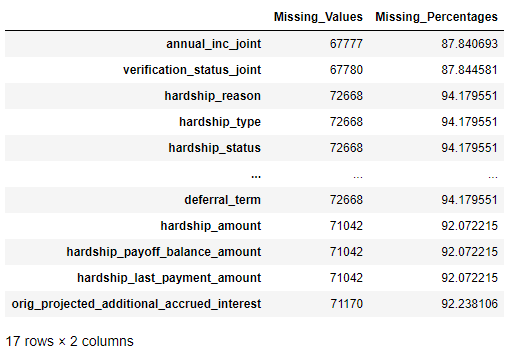
\includegraphics{MissingValues.png}
	\caption{Features having more than 6 percent missing values}
	\label{fig:MissingValues}
\end{figure}
 
\begin{table}[h!]
	\centering
	\begin{tabular}{ |p{3cm}|p{3cm}|p{3cm}|  }
		\hline
		\multicolumn{2}{|c|}{Categorical Features} \\

		\hline
		$emp\_title$ & 28185 \\
		$application\_type$ & 2 \\
		$home\_ownership$ & 5 \\
		$loan\_status$ & 7 \\
		$int\_rate$ & 129 \\
		$term$ & 2 \\
		$grade$ & 7 \\
		$earliest\_cr\_line$ & 622 \\
		$verification\_status$ & 3 \\
		$pymnt\_plan$ & 1 \\
		$purpose$ & 13 \\
		$hardship\_flag$ & 2\\
		$initial\_list\_status$ & 2\\
		$revol\_util$ & 1074 \\
		\hline
	\end{tabular}
	\caption{List of Categorical Features with unique values}
	\label{table:1}
\end{table}


\begin{figure}[h!]
	\centering
	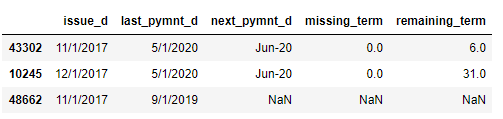
\includegraphics{dates.png}
	\caption{Transformation of Dates Columns}
	\label{fig:dates}
\end{figure}


\section{Data Preprocessing}
\subsection{Feature Engineering/Removal}
As it is discover from figure \ref{fig:MissingValues} that we have 17 features which has more than 60 percent of null values, so we have to remove them from the data. After removing those columns we left with 91 columns. After analysis i found that $id$, $emp\_title$ has more than 20000 unique values so it is better to remove them from the data. $payment\_plan$ will also be dropped because it has only  unique value. In the pre processing stage I transformed dates columns into some meaningful information like $missing\_term$, $remaining\_term$. Figure \ref{fig:dates} shows there is a pattern in these dates if we add loan term to $issue\_date$ we can get $end\_date$ and if we get the difference of $end\_date$ and $next\_pymnt\_d$ we can get $remaining\_term$. If we take difference between $next\_pymnt\_d$ and $last\_pymnt\_d$ we can calculate $missing\_term$. After creating $missing\_term$ and $remaining\_term$ I dropped the date features.

\subsection{Feature Encoding}
After some feature engineering and feature removal I encode the categorical features. As mentioned above $int\_rate$, $revol\_util$ and $term$ is converted to continuous numeric values by removing the $\%$ symbol and $month$ from the last of values. After this I still left with 7 categorical columns which needs encoding. Features like $application\_type$, $hardship\_flag$ and $initial\_list\_status$ has only two unique values so it is better to use OneHotEncoder and features like $home\_ownership$, $grade$, $purpose$ and $verification\_status$ has more than 2
 unique values so I used OrdinalEncoder for these features. I did feature encoding before the train-test split because after splitting it will increase computation I had to do encoding separately on test set. Encoding before the splitting does not expose out test set to trained model. After the encoding I split the data into train-test right before the pre processing because imputation and outlier detection might get expose our test data to models, this concept is known as Preventing data leakage in machine learning.
 
\subsection{Outlier Detection}
Outliers are the abnormal data points which may leads to bad predictions. There are number of techniques and algorithms that can be used to detect outliers. I used IsolationForest algorithm to detect outliers. Handling with outliers needs some observation if we have large number outliers than it means outliers might present some useful information. But if number of outliers are small as compare to total data we can drop them. In my case I got 6000 outliers so I drop them from data. Before applying IsolationForest I imputed the data with zero just to make isolation work. Real imputation is done after the outlier handling because this will prevent biasness from data.

\subsection{Imputation}
Imputation is another important step in data pre processing because if there are missing values in the dataset than if we try to create a model with missing values, most machine learning algorithms gives an error. As a result, you'll need to pick one of the imputation tactics. There are many techniques for the imputation of missing values in the dataset such as dropping the rows, imputing with nearest values, imputing with up and down values or imputing with mean value. For simplicity in our case Mean-imputation is used, because imputing with mean preserves the mean of that particular feature, the estimate of the mean remains unbiased whereas for the categorical feature I have missing values in $hardship\_flag$ which has 'Y' in almost more than 70 percent records so I imputed with the most frequent value in this feature. There are benefits and disadvantages of mean imputation that are not in the scope of this project.

\subsection{Normalization}
Normalization is a data transformation method that is regularly utilized in machine learning. Normalization is the way toward changing over the upsides of numeric columns in a dataset to a comparable scale without influencing the ranges of values. Many machine learning algorithms, such as support vector machines and k means, are sensitive to normalization, although many others algorithm may function without it. Also because dimensionality reduction techniques like Principle Component Analysis (PCA) are sensitive to normalization, we must do normalization before dimensionality reduction.

\subsection{Feature Selection/Dimensionality Reduction}
Dimensionality reduction is a critical step in a machine learning project since characteristics that are connected to each other produce data redundancy, which can lead to overfitting during model training. It is critical to eliminate elements that are not necessary for model training. Both the test set and the train set should have their dimensions reduced. For feature selection, a variety of methods and approaches can be applied, however correlation threshold and principle component analysis were applied in this study. We can see which features for the model training are essential via correlation, but we only get reduced dimensioned vectors via PCA. Although the outputs from both ways are different, they are both quite impressive. The most used methods for dimensionality reduction are 'Projection Methods'. The goal of projection methods is to minimise the number of dimensions in the feature space while keeping the most significant structure or connections between the variables in the data. PCA is one of the projection methods which can be good for feature reduction as correlation threshold might be contradictory to select. Comparison of the results obtain from PCA and correlation threshold will be discussed in the report later.


\section{Supervised Learning (Classification)}
\subsection{Target Class Transformation}
In the actual data we have seven different classes named as $fully\_paid$, $current$, $Late(15\ to\ 30\ days)$, $Late(30\ to\ 120\ days)$, $Grace\ Period$, $Charged\ Off$ and $default$. These classes are highly imbalance figure \ref{fig:imbalance} shows the distribution of records amongst these classes. After analysis it is concluded that $Late(15\ to\ 30\ days)$, $Late(30\ to\ 120\ days)$, $Grace\ Period$, $Charged\ Off$ and $default$ are the bad loans so I transform all these classes into a new class named as bad loan. While $fully\_paid$ remains the same as it represents that fully paid are actually good loans lastly $current$ class also remains the same as it can be either good loan or bad loan in future, so we might think these entries as loans under observation. Figure \ref{fig:new_classes} represents the distribution of target feature.
\begin{figure}[h!]
	\centering
	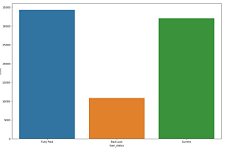
\includegraphics{classes.png}
	\caption{Transformation of target feature}
	\label{fig:new_classes}
\end{figure}

\subsection{Data Balancing}
Imbalanced data occurs when the amount of observations for all of the classes in a classification dataset is not equal. Many machine learning classifiers struggle with unbalanced training datasets because they are sensitive to the ratios of various classes. As a result, these algorithms prefer the class with the highest set of observations, which might lead to inaccurate results. This can be especially problematic when we are looking for the rare class identification since many algorithms are unable to find sufficient data for learning. We can delete entries from the majority class to balance the data, but this may result in the loss of some crucial information; another option is to add duplicate values, which is also inefficient. Our data is also highly imbalance, balancing is necessary otherwise algorithm won't have enough data for minority class for learning, so for this SMOTE technique is used, SMOTE creates new records rather than duplicating the records from the dataset which is very good for highly imbalanced data.


\subsection{Data Splitting}
I split the data at the very beginning in train-test set before any pre processing starts because it prevents the data leakage. Data leakage means test data should not be expose to the trained model. If I split data after the pre processing than there are chances that my test data get expose to the trained model. I split the data into 80 20 ratio, means 20 percent test set and 80 percent training set. For the validation I did cross validation to check whether my trained model works well on unseen data or not. Though cross-validation takes lot of processing resources so I did cross-validation only on 1 machine learning algorithm.

\subsection{Training}
The term "model training" refers to feeding data into a machine learning system so that it can generate predictions. To obtain predictions, Decision Tree, Random Forest, Adaboost are used in this study. These techniques were used twice, the first time with correlation threshold features and the second time using principle component analysis (PCA). GridSearch is used while training these machine learning algorithm so that model gets trained with good parameters this is also known as Parameter Hyper-tuning. The results from both trials are pretty impressive, with over 80$\%$ accuracy on both the test and the train set. Table \ref{table:accuracies} shows the accuracies of the models which are applied on the training set.

\begin{table}[h!]
	\centering
\begin{tabular}{ |p{3cm}|p{3cm}|p{3cm}|  }
	\hline
	\multicolumn{3}{|c|}{Models Result} \\
	\hline
	& Correlation Threshold & PCA \\
	\hline
	Decision Trees & 0.9397 &0.8532 \\
	Random Forest & 0.9309   & 0.8731 \\
	Adaboost &0.9224 & 0.8649 \\
	\hline
\end{tabular}
\caption{Training set accuracies with respect to feature reduction technique}
\label{table:accuracies}
\end{table}


\subsection{Testing}
In testing, we must examine our test data accuracies on trained models; in this study, I feed test data to our trained models to obtain test data predictions. Models trained using PCA provide more than 80 percent accuracy on the test set, whereas models trained with correlation threshold provide more than 90 percent accuracy on the test set. Table \ref{table:accuracies} shows the overall accuracy of the test sets on the trained models.
\begin{table}[h!]
	\centering
	\begin{tabular}{ |p{3cm}|p{3cm}|p{3cm}|  }
		\hline
		\multicolumn{3}{|c|}{Models Test Set Results} \\
		\hline
		& Correlation Threshold & PCA \\
		\hline
		Decision Trees & 0.9406 &0.8101 \\
		Random Forest & 0.9428   & 0.8396 \\
		Adaboost &0.9375 & 0.8545 \\
		\hline
	\end{tabular}
	\caption{Test set accuracies with respect to feature reduction technique}
	\label{table:test_accuracies}
\end{table}

\subsection{Experiment Comparison and Evaluation}
Table \ref{table:correlation_results} and table \ref{table:pca_results} shows the experiment results and findings of different algorithms applied with different feature reduction methods. By looking at the tables it can be seen that adaboost works well with Principle Component Analysis and with Correlation threshold as compare to other algorithms. Other algorithms like decision tree, random forest also has the overall accuracy of 94 percent and recall for minor class is just above the 60 percent with correlation threshold which is also impressive. With PCA decision tree, random forest has the overall accuracy of 81 percent and 84 percent and recall for minor class is approximately 80 percent. As our data is quite imbalance so accuracy might not be the good measure to evaluate model, if our recall for minority class is good than we can say that our model performs well on test data. Recall tells the percentage of correctly predicted values of a particular class so if our minority class records are correctly identify by the model than we can say that model is working good on the test data. 
\begin{table}[h!]
	\centering
	\begin{tabular}{ |p{3cm}||p{2cm}|p{2cm}|p{2cm}|p{2cm}|  }
		\hline
		\multicolumn{5}{|c|}{Correlation Threshold Results} \\
		\hline
		& Target Class & Precision & Recall & Overall Accuracy \\
		\hline
		Adaboost & Fully Paid & 0.91 & 0.99 & 0.94\\
					  & Bad Loan & 0.95   & 0.63 & \\
					  & Current &0.96 & 0.98 & \\
		\hline
		Decision Tree & Fully Paid & 0.92 & 0.99 & 0.94\\
		& Bad Loan & 0.92 &  0.62 & \\
		& Current &0.97 & 0.99 & \\
		\hline
		Random Forest & Fully Paid & 0.92  & 1.00 & 0.94\\
		& Bad Loan & 0.98  &  0.61 & \\
		& Current & 0.96   &   1.00 & \\
		\hline
	\end{tabular}
	\caption{Correlation Results}
	\label{table:correlation_results}
\end{table}




\begin{table}[h!]
	\centering
	\begin{tabular}{ |p{3cm}||p{2cm}|p{2cm}|p{2cm}|p{2cm}|  }
		\hline
		\multicolumn{5}{|c|}{PCA Results} \\
		\hline
		& Target Class & Precision & Recall & Overall Accuracy \\
		\hline
		Adaboost & Fully Paid &0.86 & 0.88 & 0.85\\
		& Bad Loan & 0.86 & 0.81 & \\
		& Current & 0.85 & 0.84 & \\
		\hline
		Decision Tree & Fully Paid & 0.80 & 0.84 & 0.81\\
		& Bad Loan & 0.85 &  0.80 & \\
		& Current &0.81 &  0.78 & \\
		\hline
		Random Forest & Fully Paid & 0.82 & 0.88 & 0.84\\
		& Bad Loan &0.98  & 0.79 & \\
		& Current & 0.83 & 0.81 & \\
		\hline
	\end{tabular}
	\caption{PCA Results}
	\label{table:pca_results}
\end{table}

\section{Unsupervised Learning (Clustering)}
For the unsupervised learning I took the entire data, pre processed that data with similar techniques as I did in classification but feature reduction is done by some projection methods like PCA, FAMD. Like classification I did some comparative study tried to predict clusters under different scenarios. I use K-MEANS with some dimensionality reduction methods and K-Prototype which is a advance version of K-MEANS.
\subsection{Issue with data for clustering}
As our dataset contains some categorical information so applying K-MEANS directly on the data will not work because K-MEANS work by calculating the distance so K-MEAN consider our encoded categorical features as continuous numeric value but in reality these encoded features are discrete values. To overcome this problem I use projection methods like PCA, FAMD for dimensionality reduction. Factor analysis of mixed data types (FAMD) excepts data with continuous numeric values and categorical values and produce the reduced dimensioned data. Except K-MEANS with projection methods I also applied K-Prototype which is latest version of KMEANS which deal with categorical features on its own, it calculates the distance differently on categorical features as compare to numerical feature.


\subsection{Elbow Scoring and Silhouette Scoring}
Elbow methods helps to calculate the optimal number of clusters for clustering algorithm. I applied elbow method for K-MEANS after reducing the data dimensionality with PCA and FAMD. After determining the number of optimal cluster we have to check the Silhouette score which is a matrix used to check the goodness of the clusters. Figure \ref {fig:scores} shows silhouette scores with clusters from 2 to 5 for PCA and FAMD reduced data
%\begin{figure}[h!]
%	\centering
%	\includegraphics{pca_elbow.png}
%	\caption{Elbow method estimation for PCA reduced data}
%	\label{fig:elbow_result}
%\end{figure}
%\begin{figure}[h!]
%	\centering
%	\subfloat[\centering Elbow method estimation for FAMD reduced data %]{{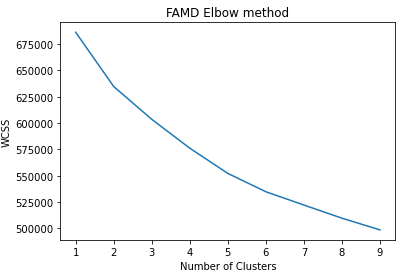
\includegraphics[width=7cm]{famd_elbow} }}%
%	\qquad
%	\subfloat[\centering Elbow method estimation for PCA reduced %data]{{\includegraphics[width=7cm]{pca_elbow} }}%
%	\caption{Elbow method estimation for FAMD and PCA Data}%
%	\label{fig:elbow_result}%
%\end{figure}

.
%\begin{figure}[h!]
%	\centering
%	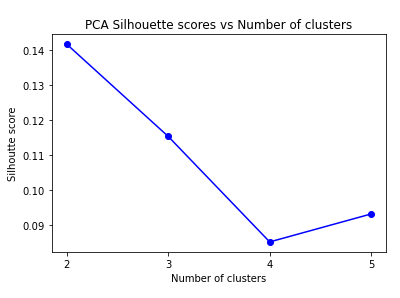
\includegraphics{pca_score.png}
%	\caption{Silhouette Scores for the PCA reduced data}
%	\label{fig:scores}
%\end{figure}
\begin{figure}[h!]
	\centering
	\subfloat[\centering Silhouette Scores for the FAMD reduced data ]{{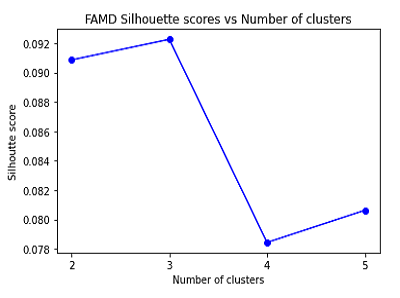
\includegraphics[width=7cm]{famd_scores} }}%
	\qquad
	\subfloat[\centering  Silhouette Scores for the PCA reduced data]{{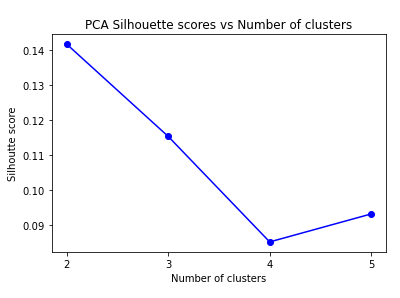
\includegraphics[width=7cm]{pca_score} }}%
	\caption{Silhouette scores for the FAMD and PCA reduced data}%
	\label{fig:scores}%
\end{figure}

After observing figure \ref{fig:scores} it can be seen that the best optimal silhouette score is 0.14 for PCA reduced data with 2 clusters which is highest in both graphs. So for good predictions it is better to apply K-MEANS with 2 clusters on PCA reduced data.

\subsection{K-MEANS}
After getting the data which is transformed by PCA we has no discrete values in the data and optimal number of clusters from elbow method and silhouette score we can apply K-MEANS. I applied K-MEANS on PCA reduced data with 2 clusters to get predictions, the results of the K-MEAN with 2 clusters are shown in figure \ref{fig:kmeans_result_2d}. By looking at figure \ref{fig:kmeans_result_2d} it can clearly seen that our data has a definite pattern. 


\subsection{Experiment with other algorithm}
K-Prototypes is a lesser-known versoin of K-MEANS that has the benefit of working with a variety of data types. It uses Euclidean distance (like K-means) to assess distance between numerical features, but it also uses the number of matching categories to evaluate distance between categorical data. I applied K-Prototype to the original data which has categorical and numerical values in it. As it has categorical values so scoring for the K-Protoype is difficult to get, it requires some mathematics, which is not in the scope of this study. I applied K-Prototype just to visualize that whether our data shows some pattern with algorithms other than K-MEANS. The experiment results with K-Prototype is shown in the figure \ref{fig:k_pro_re}
\begin{figure}[h!]
	\centering
	\subfloat[\centering PCA reduced data K-MEANS clusters in 3d Scatter plot]{{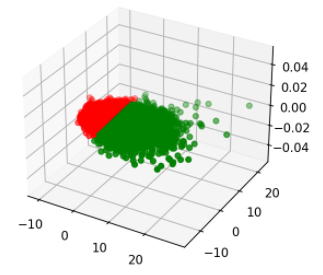
\includegraphics[width=7cm]{pca_3d} }}%
	\qquad
	\subfloat[\centering PCA reduced data K-MEANS clusters in 2d Scatter plot]{{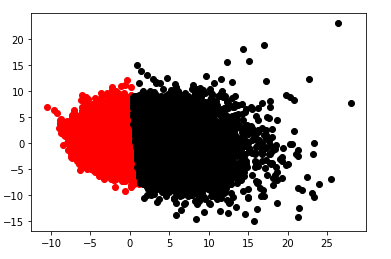
\includegraphics[width=7cm]{pca_2d} }}%
	
	\caption{K-MEANS Prediction PCA Data}%
	\label{fig:kmeans_result_2d}%
\end{figure}

\begin{figure}[h!]
	\centering
	\subfloat[\centering PCA reduced data K-MEANS clusters in 3d Scatter plot]{{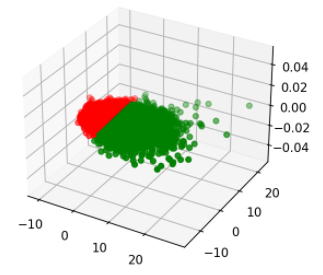
\includegraphics[width=7cm]{pca_3d} }}%
	\qquad
	\subfloat[\centering PCA reduced data K-MEANS clusters in 2d Scatter plot]{{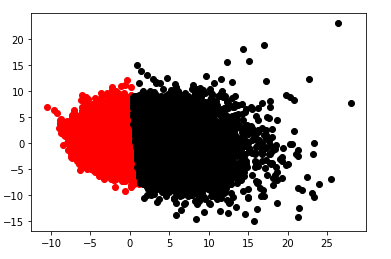
\includegraphics[width=7cm]{pca_2d} }}%
	
	\caption{K-Prototypes Predictions}%
	\label{fig:k_pro_re}%
\end{figure}


\section{Conclusion}


\singlespacing

\bibliographystyle{agsm}
\bibliography{document}

\end{document}




